% Rapport -- TP Techniques de compilation : du texte d'une expression régulière à l'automate
% Compiler avec pdfLaTeX (compilateur par défaut d'Overleaf).
\documentclass[12pt,a4paper]{article}

% ---------------------------------------------------------------- encodage, langue
\usepackage[utf8]{inputenc}
\usepackage[T1]{fontenc}
\IfFileExists{french.ldf}{%
  \usepackage[french]{babel}
  \frenchsetup{AutoSpacePunctuation=false, StandardItemLabels=true, StandardLists=true}
}{\usepackage[english]{babel}}

% ---------------------------------------------------------------- polices (consignes de remise)
% Texte : Times New Roman 12 ; titres : 14 ; code : Courier New 10.
% pdfLaTeX (défaut d'Overleaf) : Times et Courier (clones PostScript standard).
% XeLaTeX / LuaLaTeX : vraies polices Times New Roman / Courier New si installées.
\usepackage{iftex}
\usepackage{mathptmx}
\ifPDFTeX
  \renewcommand{\ttdefault}{pcr}
\else
  \usepackage[no-math]{fontspec}
  \IfFontExistsTF{Times New Roman}{\setmainfont{Times New Roman}}{\setmainfont{TeX Gyre Termes}}
  \IfFontExistsTF{Courier New}{\setmonofont{Courier New}}{\setmonofont{TeX Gyre Cursor}}
\fi
\linespread{1}
\usepackage{amsmath,amssymb}
\usepackage{microtype}
\usepackage[a4paper,margin=2.5cm,headheight=15pt]{geometry}
\usepackage{xcolor}
\definecolor{bleu}{HTML}{1F3B5C}
\definecolor{bleuclair}{HTML}{2E5A88}
\definecolor{fondcode}{HTML}{F4F6F9}
\definecolor{gris}{HTML}{6B7280}
\usepackage{titlesec}
\titleformat{\section}{\fontsize{14}{17}\selectfont\bfseries\color{bleu}}{\thesection.}{0.5em}{}
\titleformat{\subsection}{\fontsize{14}{17}\selectfont\bfseries\color{bleuclair}}{\thesubsection}{0.6em}{}
\titlespacing*{\section}{0pt}{1.6ex plus .5ex}{0.8ex}
\titlespacing*{\subsection}{0pt}{1.2ex plus .4ex}{0.5ex}
\usepackage{fancyhdr}
\pagestyle{fancy}
\fancyhf{}
\fancyhead[L]{\small\color{gris}TP Techniques de compilation}
\fancyhead[R]{\small\color{gris}De l'expression r\'eguli\`ere \`a l'automate}
\fancyfoot[C]{\small\thepage}
\renewcommand{\headrulewidth}{0.4pt}

% ---------------------------------------------------------------- tableaux, listes, figures
\usepackage{booktabs,tabularx,array}
\usepackage{enumitem}
\setlist{itemsep=2pt,topsep=3pt}
\usepackage{graphicx}
\usepackage[font=small,labelfont={bf,color=bleu},labelsep=endash]{caption}
\usepackage{float}
\usepackage{forest}
\usepackage[most]{tcolorbox}
\usepackage[hidelinks]{hyperref}

% ---------------------------------------------------------------- code
\usepackage{listings}
\lstdefinestyle{base}{
  basicstyle=\ttfamily\fontsize{10}{12}\selectfont, columns=fixed, basewidth=0.6em, keepspaces=true,
  backgroundcolor=\color{fondcode}, frame=leftline, rulecolor=\color{bleuclair},
  framerule=1.2pt, xleftmargin=6pt, framexleftmargin=4pt, aboveskip=6pt, belowskip=6pt,
  extendedchars=false, upquote=true, breaklines=true,
  literate={->}{{$\rightarrow$}}2 {EPS}{{$\varepsilon$}}1 {′}{{$'$}}1 {ε}{{$\varepsilon$}}1 {→}{{$\rightarrow$}}1 {é}{{\'e}}1
           {è}{{\`e}}1 {à}{{\`a}}1 {…}{{\ldots}}1 {×}{{$\times$}}1
}
\lstdefinestyle{schema}{style=base}
\lstdefinestyle{py}{style=base, language=Python,
  keywordstyle=\color{bleu}\bfseries, commentstyle=\color{gris}\itshape,
  stringstyle=\color{teal!70!black}}

% ---------------------------------------------------------------- macros
\newcommand{\code}[1]{{\fontsize{10}{12}\selectfont\texttt{#1}}}
\newcommand{\eps}{\ensuremath{\varepsilon}}
\newcommand{\Prem}{\textsc{Premier}}
\newcommand{\Suiv}{\textsc{Suivant}}
\newcommand{\fr}[2]{\ensuremath{[#1\to#2]}}
\newcommand{\tok}[1]{\ensuremath{\text{\fontsize{10}{12}\selectfont\ttfamily #1}}}
\newtcolorbox{afaire}{colback=yellow!12, colframe=orange!70!black, boxrule=0pt,
  leftrule=3pt, arc=0pt, left=6pt, right=6pt, top=3pt, bottom=3pt, fontupper=\small\color{orange!40!black}}
\newcolumntype{L}{>{\raggedright\arraybackslash}X}
\newcolumntype{C}{>{\centering\arraybackslash}p}

\setlength{\emergencystretch}{4em}

\begin{document}

% ================================================================ page de garde
\begin{titlepage}
\centering
\vspace*{1.2cm}
{\fontsize{14}{17}\selectfont\color{gris} 3\textsuperscript{e} année Ingénieur Informatique --- Techniques de compilation\par}
\vspace{2.2cm}
{\color{bleu}\rule{\linewidth}{1pt}\par}
\vspace{0.5cm}
{\fontsize{24}{29}\selectfont\bfseries\color{bleu} TP Techniques de compilation\par}
\vspace{0.4cm}
{\fontsize{18}{22}\selectfont\color{bleu} Du texte d'une expression régulière à l'automate\par}
\vspace{0.3cm}
{\fontsize{12}{15}\selectfont\itshape Traduction dirigée par la syntaxe et grammaires attribuées\par}
\vspace{0.5cm}
{\color{bleu}\rule{\linewidth}{1pt}\par}
\vspace{1.2cm}
{\fontsize{14}{17}\selectfont Année universitaire 2026--2027\par}
\vspace{0.3cm}
{Rapport rendu le 25 novembre 2026 --- Langage : Python 3\par}
\vspace{1.6cm}
{\fontsize{14}{17}\selectfont\bfseries\color{bleu} Identification de l'équipe et fiche de répartition\par}
\vspace{0.4cm}
{\small
\begin{tabularx}{\linewidth}{>{\raggedright\arraybackslash}p{3.6cm} L >{\raggedright\arraybackslash}p{3.4cm}}
\toprule
Nom et prénom & Parties en charge & Parties relues \\
\midrule
ISSAOUI Edem & Étudiant 1 : analyse lexicale, partie 1 (grammaire LL(1), \Prem/\Suiv, table), partie 2 (analyseur prédictif) & Partie 4, tests, rapport \\ \addlinespace
BEN TAHER Houssem & Étudiant 2 : partie 3 (schéma de traduction, constructions de Thompson) & Parties 1 et 2 \\ \addlinespace
JAZIRI Yahia & Étudiant 3 : partie 5 (export Graphviz, simulation, interface en ligne de commande) & Partie 3 \\ \addlinespace
MTAWA Bara & Étudiant 4 : partie 4 (numérotation des états), partie 6 (jeu de tests), rapport, correction de \tok{+} et \tok{?} & Partie 5 \\
\bottomrule
\end{tabularx}\par}
\vfill
\end{titlepage}

\setcounter{page}{1}

% ================================================================ présentation et apport
\section*{Présentation et apport de l'équipe}

Le traducteur est écrit en Python 3, sans générateur d'analyseur ni bibliothèque d'expressions
régulières. \code{src/} contient l'analyseur lexical, l'analyseur prédictif (une procédure par
non-terminal, portant les actions sémantiques), les constructeurs de Thompson, la simulation,
l'export \code{.dot} et l'interface en ligne de commande. Un fragment est un triplet
\code{(init, fin, transitions)} ; l'étiquette \code{None} représente \eps.

\textbf{Notre apport.} En vérifiant les automates sur tous les mots courts, nous avons découvert
que la première construction de \tok{+} et \tok{?} était fausse (\code{(ab+)?} acceptait
\code{b}) ; nous l'avons corrigée (sections~\ref{sec:constructeurs} et~\ref{sec:difficultes}), et
l'automate a désormais \textbf{exactement $\boldsymbol{2n}$ états}. La numérotation circule comme un
attribut, sans compteur global. Le jeu de tests ajoute trois cas limites, dix tests d'erreur et un
contrôle automatique de la borne $2n$ et de l'invariant sur 506 expressions ; il détecte le défaut
de la première version. Aucune extension facultative n'a
été réalisée.

% ================================================================ PARTIE 1
\section{Partie 1 --- Grammaire LL(1)}

\subsection{\Prem{}, \Suiv{} et table d'analyse prédictive}

\begin{table}[H]
\centering\small
\begin{tabular}{c c l l}
\toprule
 & Annulable & \Prem & \Suiv \\
\midrule
$R$  & non & \tok{( SYMBOLE @}      & \tok{) \$} \\
$R'$ & oui & \tok{|} \eps            & \tok{) \$} \\
$T$  & non & \tok{( SYMBOLE @}      & \tok{| ) \$} \\
$T'$ & oui & \tok{( SYMBOLE @} \eps  & \tok{| ) \$} \\
$F$  & non & \tok{( SYMBOLE @}      & \tok{( SYMBOLE @ | ) \$} \\
$F'$ & oui & \tok{* + ?} \eps        & \tok{( SYMBOLE @ | ) \$} \\
$A$  & non & \tok{( SYMBOLE @}      & \tok{* + ? ( SYMBOLE @ | ) \$} \\
\bottomrule
\end{tabular}
\caption{Ensembles \Prem{} et \Suiv{}.}
\end{table}

\begin{table}[H]
\centering\small
\setlength{\tabcolsep}{5pt}
\begin{tabular}{c|ccccccccc}
\toprule
 & \tok{(} & \tok{SYMBOLE} & \tok{@} & \tok{|} & \tok{*} & \tok{+} & \tok{?} & \tok{)} & \tok{\$} \\
\midrule
$R$  & $T R'$ & $T R'$ & $T R'$ & & & & & & \\
$R'$ & & & & $\texttt{|}\,T R'$ & & & & \eps & \eps \\
$T$  & $F T'$ & $F T'$ & $F T'$ & & & & & & \\
$T'$ & $F T'$ & $F T'$ & $F T'$ & \eps & & & & \eps & \eps \\
$F$  & $A F'$ & $A F'$ & $A F'$ & & & & & & \\
$F'$ & \eps & \eps & \eps & \eps & $\texttt{*}F'$ & $\texttt{+}F'$ & $\texttt{?}F'$ & \eps & \eps \\
$A$  & $\texttt{(}R\texttt{)}$ & \tok{SYMBOLE} & \tok{@} & & & & & & \\
\bottomrule
\end{tabular}
\caption{Table LL(1) ; une case vide est une erreur.}
\end{table}

\textbf{Absence de conflit.} Pour chaque non-terminal à plusieurs règles, les ensembles de
sélection sont disjoints : $R'$ : $\{\texttt{|}\}$ et $\{\texttt{)},\texttt{\$}\}$ ; $T'$ :
$\Prem(F)$ et $\{\texttt{|},\texttt{)},\texttt{\$}\}$ ; $F'$ : $\{\texttt{*}\}$, $\{\texttt{+}\}$,
$\{\texttt{?}\}$ et $\Suiv(F')$ ; $A$ : trois terminaux distincts. La grammaire est LL(1).

\subsection{Question 1 --- Grammaire de départ, transformation et concaténation implicite}

\textbf{Grammaire de départ.} La grammaire fournie est issue de la grammaire naturelle, récursive
à gauche, qui traduit directement la priorité \tok{|} $<$ concaténation $<$ postfixés et
l'associativité à gauche de l'union et de la concaténation :
\[
R \to R\;\texttt{|}\;T \mid T \qquad T \to T\,F \mid F \qquad
F \to F\,\texttt{*} \mid F\,\texttt{+} \mid F\,\texttt{?} \mid A \qquad
A \to \texttt{(}\,R\,\texttt{)} \mid \texttt{SYMBOLE} \mid \texttt{@}
\]

\textbf{Transformation appliquée.} Une analyse descendante ne peut pas traiter une règle
récursive à gauche : la procédure de $R$ appellerait $R$ sans consommer de jeton et bouclerait
indéfiniment. On élimine cette récursivité par la transformation classique
\[
X \to X\,\alpha \mid \beta \quad\Longrightarrow\quad X \to \beta\,X', \qquad X' \to \alpha\,X' \mid \varepsilon,
\]
avec $\alpha = \texttt{|}\,T$, $\beta = T$ pour $R$ ; $\alpha = F$, $\beta = F$ pour $T$ ; $\alpha
\in \{\texttt{*}, \texttt{+}, \texttt{?}\}$, $\beta = A$ pour $F$. On obtient exactement $R'$,
$T'$ et $F'$ de la grammaire fournie, et le langage reconnu est inchangé.

\textbf{Pourquoi tester \Prem(\textit{F}) dans \textit{T}'.} La concaténation est
implicite : aucun symbole ne sépare $r$ et $s$ dans $rs$. Pour choisir entre $T' \to F\,T'$
(un facteur de plus) et $T' \to \varepsilon$ (fin de la concaténation), le seul indice est le
jeton courant : on continue si et seulement s'il peut commencer un facteur, c'est-à-dire s'il
appartient à $\Prem(F) = \{\texttt{(}, \texttt{SYMBOLE}, \texttt{@}\}$. Ce choix est
déterministe car $\Prem(F)$ est disjoint de $\Suiv(T') = \{\texttt{|}, \texttt{)}, \texttt{\$}\}$ :
un \tok{|} ou une \tok{)} ne peut jamais débuter un facteur et signale la fin de la
concaténation en cours.

\subsection{Question 2 --- Détection des erreurs de \texttt{a)} et de \texttt{a||b}}

Les positions sont comptées à partir de 0, la fin de l'entrée étant à la position
\code{len(texte)}.
\begin{itemize}
\item \textbf{\texttt{a)}} : l'analyse de \code{a} réussit. Sur \tok{)}, $F'$, $T'$ puis $R'$
  choisissent \eps{} (cases $M[F', \texttt{)}]$, $M[T', \texttt{)}]$, $M[R', \texttt{)}]$), ce qui
  est légitime puisque \tok{)} appartient à leur \Suiv{} (elle peut suivre $R$ entre
  parenthèses). $R$ se termine donc normalement, mais un jeton reste non consommé : l'erreur est
  détectée \textbf{après l'analyse de $\boldsymbol{R}$, au test de fin d'entrée} (en version
  tabulaire : sommet de pile \tok{\$} face au jeton \tok{)}), à la position 1, avec « fin de
  l'expression » attendue.
\item \textbf{\texttt{a||b}} : $R'$ lit le premier \tok{|} (case $M[R', \texttt{|}]$) puis appelle
  $T$ avec le second \tok{|} comme jeton courant. La \textbf{case $\boldsymbol{M[T,
  \texttt{|}]}$ est vide} : l'erreur est détectée à la position 2, avec \tok{(}, un symbole ou
  \tok{@} attendus.
\end{itemize}
% ================================================================ PARTIE 3
\section{Partie 3 --- Schéma de traduction prédictif}

\subsection{Schéma complet}
$X.h$ est le fragment déjà construit à gauche (hérité), $X.s$ le résultat (synthétisé) ;
chaque action est placée là où elle s'exécute dans la procédure (figure~\ref{fig:schema}).

\begin{figure}[htb]
\begin{lstlisting}[style=schema]
R  -> T  { R'.h := T.s }  R'  { R.s := R'.s }
R' -> '|' T  { R'1.h := union(R'.h, T.s) }  R'1  { R'.s := R'1.s }
R' -> EPS  { R'.s := R'.h }
T  -> F  { T'.h := F.s }  T'  { T.s := T'.s }
T' -> F  { T'1.h := concat(T'.h, F.s) }  T'1  { T'.s := T'1.s }
T' -> EPS  { T'.s := T'.h }
F  -> A  { F'.h := A.s }  F'  { F.s := F'.s }
F' -> '*' { F'1.h := etoile(F'.h) } F'1 { F'.s := F'1.s }
F' -> '+' { F'1.h := plus(F'.h) }   F'1 { F'.s := F'1.s }
F' -> '?' { F'1.h := option(F'.h) } F'1 { F'.s := F'1.s }
F' -> EPS  { F'.s := F'.h }
A  -> '(' R ')'  { A.s := R.s }
A  -> SYMBOLE    { A.s := symbole(SYMBOLE.val) }
A  -> '@'        { A.s := vide() }
\end{lstlisting}
\caption{Schéma de traduction complet.}\label{fig:schema}
\end{figure}

\subsection{Constructeurs de Thompson, dont \texttt{+} et \texttt{?}}\label{sec:constructeurs}

\begin{table}[H]
\centering\small
\begin{tabularx}{\linewidth}{l c L}
\toprule
Constructeur & États & Transitions ajoutées (\eps{} sauf indication) \\
\midrule
\code{symbole(a)}, \code{vide()} & $i, f$ & $i \xrightarrow{a} f$ (resp. $i \xrightarrow{\varepsilon} f$) \\
\code{union(r, s)}  & $i, f$ & $i \to \mathrm{init}(r), \mathrm{init}(s)$ ; $\mathrm{fin}(r), \mathrm{fin}(s) \to f$ \\
\code{concat(r, s)} & aucun  & $\mathrm{fin}(r) \to \mathrm{init}(s)$ \\
\code{etoile(r)}    & $i, f$ & $i \to \mathrm{init}(r)$, $\mathrm{fin}(r) \to f$, $\mathrm{fin}(r) \to \mathrm{init}(r)$, $i \to f$ \\
\code{plus(r)}      & $i, f$ & comme l'étoile, sans $i \to f$ \\
\code{option(r)}    & $i, f$ & comme l'étoile, sans la boucle $\mathrm{fin}(r) \to \mathrm{init}(r)$ \\
\bottomrule
\end{tabularx}
\caption{Constructeurs utilisés par les actions sémantiques.}
\end{table}

$r^+ = r\,r^*$ demanderait deux exemplaires de $N(r)$. Or, dans $N(r^*)$, seule l'arête
$i \to f$ évite $N(r)$ : sans elle, on obtient exactement $r^+$ avec un seul exemplaire.
$r? = r \mid \varepsilon$ : l'union avec $N(\varepsilon)$ se réduit à l'arête $i \to f$, soit
l'étoile sans la boucle. Dans les deux cas, $i$ n'a pas de transition entrante ni $f$ de
transition sortante : l'invariant de Thompson est conservé. Chaque élément compté (symbole,
\tok{@}, \tok{|}, \tok{*}, \tok{+}, \tok{?}) crée deux états et la concaténation aucun :
l'automate a \textbf{exactement $\boldsymbol{2n}$ états}.

\subsection{Graphe de dépendances de \texttt{ab|c}}

\begin{figure}[tb]
\centering
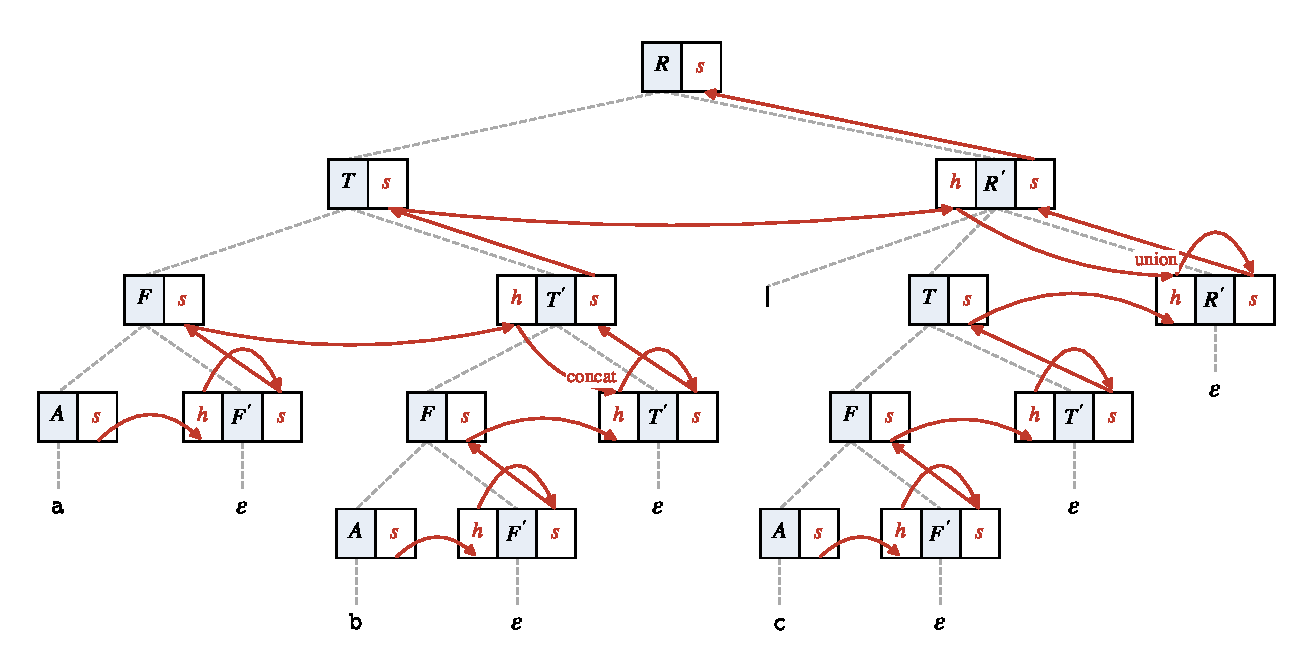
\includegraphics[width=0.78\linewidth]{figures/dep.pdf}
\caption{Arbre de \code{ab|c} (pointillés) et dépendances entre attributs (flèches rouges).}
\label{fig:dep}
\end{figure}

Dans chaque règle $X \to Y_1 \dots Y_k$, un attribut hérité de $Y_i$ ne dépend que de $X.h$ et
d'attributs de $Y_1 \dots Y_{i-1}$ (ex. $R'_1.h := \mathrm{union}(R'.h, T.s)$ : père et frère
gauche). Le schéma est donc \textbf{L-attribué} et s'évalue en une passe pendant la descente. Il
n'est \textbf{pas S-attribué} : les attributs hérités sont indispensables, car dans
$R' \to \texttt{|}\,T\,R'_1$ l'opérande gauche de l'union n'est pas dans le sous-arbre de $R'$.

\subsection{Arbre annoté de \texttt{a|bc*}}

\begin{figure}[H]
\centering
\resizebox{0.64\linewidth}{!}{%
\begin{forest}
  for tree={
    font=\footnotesize, align=center, inner sep=2.5pt, draw=bleuclair, rounded corners=1pt,
    fill=fondcode, l sep=6pt, s sep=6pt, edge={gris}, parent anchor=south, child anchor=north
  },
  leaf/.style={draw=none, fill=none, font=\small\ttfamily}
  [{$R$\\ $s{=}\fr{8}{9}$\\ nh=0 ns=10}
    [{$T$\\ $s{=}\fr{0}{1}$\\ nh=0 ns=2}
      [{$F$\\ $s{=}\fr{0}{1}$\\ nh=0 ns=2}
        [{$A$\\ $s{=}\fr{0}{1}$\\ nh=0 ns=2} [a, leaf]]
        [{$F'$\\ $h{=}\fr{0}{1}$\\ $s{=}\fr{0}{1}$\\ nh=2 ns=2} [\eps, leaf]]]
      [{$T'$\\ $h{=}\fr{0}{1}$\\ $s{=}\fr{0}{1}$\\ nh=2 ns=2} [\eps, leaf]]]
    [{$R'$\\ $h{=}\fr{0}{1}$\\ $s{=}\fr{8}{9}$\\ nh=2 ns=10}
      [|, leaf]
      [{$T$\\ $s{=}\fr{2}{7}$\\ nh=2 ns=8}
        [{$F$\\ $s{=}\fr{2}{3}$\\ nh=2 ns=4}
          [{$A$\\ $s{=}\fr{2}{3}$\\ nh=2 ns=4} [b, leaf]]
          [{$F'$\\ $h{=}\fr{2}{3}$\\ $s{=}\fr{2}{3}$\\ nh=4 ns=4} [\eps, leaf]]]
        [{$T'$\\ $h{=}\fr{2}{3}$\\ $s{=}\fr{2}{7}$\\ nh=4 ns=8}
          [{$F$\\ $s{=}\fr{6}{7}$\\ nh=4 ns=8}
            [{$A$\\ $s{=}\fr{4}{5}$\\ nh=4 ns=6} [c, leaf]]
            [{$F'$\\ $h{=}\fr{4}{5}$\\ $s{=}\fr{6}{7}$\\ nh=6 ns=8}
              [*, leaf]
              [{$F'$\\ $h{=}\fr{6}{7}$\\ $s{=}\fr{6}{7}$\\ nh=8 ns=8} [\eps, leaf]]]]
          [{$T'$\\ $h{=}\fr{2}{7}$\\ $s{=}\fr{2}{7}$\\ nh=8 ns=8} [\eps, leaf]]]]
      [{$R'$\\ $h{=}\fr{8}{9}$\\ $s{=}\fr{8}{9}$\\ nh=10 ns=10} [\eps, leaf]]]]
\end{forest}}
\caption{Arbre annoté de \code{a|bc*} ; fragment noté $[\mathrm{init}\to\mathrm{fin}]$, nh/ns : $n$ et $n'$ (partie~4).}
\label{fig:arbre}
\end{figure}

\code{a} donne \fr01, \code{b} \fr23, \code{c} \fr45, l'étoile \fr67 ; $T'$ concatène \fr23 et
\fr67 en \fr27, puis l'union crée \fr89, qui remonte jusqu'à $R.s$.

\subsection{Associativité et opérateur délicat}

Bien que $R' \to \texttt{|}\,T\,R'$ soit récursive à droite, l'attribut hérité transporte vers la
droite ce qui est déjà construit : pour \code{a|b|c}, $R'$ calcule
$\mathrm{union}(N(a), N(b)) = \fr45$, puis $\mathrm{union}(\fr45, N(c)) = \fr89$, soit
\code{(a|b)|c}. Des attributs seulement synthétisés auraient donné \code{a|(b|c)}.

L'opérateur le plus délicat est \tok{+} : $r^+ = r\,r^*$ mentionne $r$ deux fois ; réutiliser
$N(r)$ placerait les mêmes états à deux endroits, le recopier casserait la borne $2n$, et ajouter
la boucle sur les états de $N(r)$ fausse l'automate (section~\ref{sec:difficultes}).

% ================================================================ PARTIE 4
\section{Partie 4 --- Numérotation des états sans variable globale}\label{sec:partie4}

Le prochain numéro libre devient un attribut : $X.n$ (hérité) est le premier numéro libre avant
l'analyse de $X$, $X.n'$ (synthétisé) le premier numéro libre après. $R.n := 0$ et $R.n'$ est le
nombre total d'états. Chaque constructeur reçoit $n$ ; symbole, vide, union, étoile, plus et
option numérotent $n$ et $n+1$ et rendent $n+2$, la concaténation rend $n$. Le schéma de la
partie~3 est complété ainsi (règles représentatives) :

\noindent\begin{minipage}{\linewidth}
\begin{lstlisting}[style=schema]
R  -> { T.n := R.n } T { R'.h := T.s ; R'.n := T.n' }
       R' { R.s := R'.s ; R.n' := R'.n' }
R' -> '|' { T.n := R'.n } T
       { (R'1.h, R'1.n) := union(R'.h, T.s, T.n') }
       R'1 { R'.s := R'1.s ; R'.n' := R'1.n' }
F' -> '*' { (F'1.h, F'1.n) := etoile(F'.h, F'.n) }
       F'1 { F'.s := F'1.s ; F'.n' := F'1.n' }
A  -> SYMBOLE { (A.s, A.n') := symbole(SYMBOLE.val, A.n) }
\end{lstlisting}
\end{minipage}

$T$, $T'$ et $F$ suivent le modèle de $R$ et $R'$ (avec \code{concat}), \tok{+} et \tok{?} celui de
\tok{*}, \tok{@} celui de \code{SYMBOLE}, et chaque règle \eps{} pose $X.n' := X.n$. Le schéma
reste L-attribué. Dans le code, $n$ est un paramètre de chaque procédure et $n'$ fait partie de sa
valeur de retour : \code{R(n) -> (s, n')}, \code{Rp(h, n) -> (s, n')}, et \code{parse()} appelle
\code{R(0)}. Aucune variable globale ni attribut d'objet ne sert de compteur : chaque analyse repart
de 0.

\textbf{Invariant.} Si $X$ est appelé avec $n$ et rend $(s, n')$, les états de $s$ sont
exactement $n, \dots, n'-1$ et $n' - n = 2k$, où $k$ est le nombre d'éléments comptés lus par
$X$. Par récurrence : une feuille crée $\{n, n+1\}$ ; une union, une étoile, un \tok{+} ou un
\tok{?} ajoutent deux numéros juste après ceux de leurs opérandes ; la concaténation et les règles
\eps{} n'ajoutent rien. Aucun état n'est donc réutilisé et l'automate a exactement $2n$ états
numérotés de 0 à $2n-1$. Pour \code{a|bc*} (figure~\ref{fig:arbre}), $R.n' = 10 = 2 \times 5$.

% ================================================================ PARTIE 5
\section{Partie 5 --- Export Graphviz, simulation et automates générés}\label{sec:partie5}

\code{graphviz\_export.py} produit le fichier \code{.dot} : graphe de gauche à droite, flèche
d'entrée vers l'état initial, double cercle pour l'état final, étiquette \eps{} explicite, et
transitions parallèles regroupées (\code{a,b}). \code{simulation.py} range les transitions une fois
dans des dictionnaires, puis part de l'\eps-fermeture de l'état initial, suit chaque caractère et
recalcule la fermeture ; le mot est accepté si l'état final est atteint. La fermeture mémorise les
états visités (terminaison sur les cycles d'\eps{}) ; coût $O(m\,(V+E))$. Sept automates (\code{.dot} et \code{.png}) sont fournis dans
\code{automates/} ; les commandes sont dans \code{README.txt}.

\begin{figure}[H]
\centering
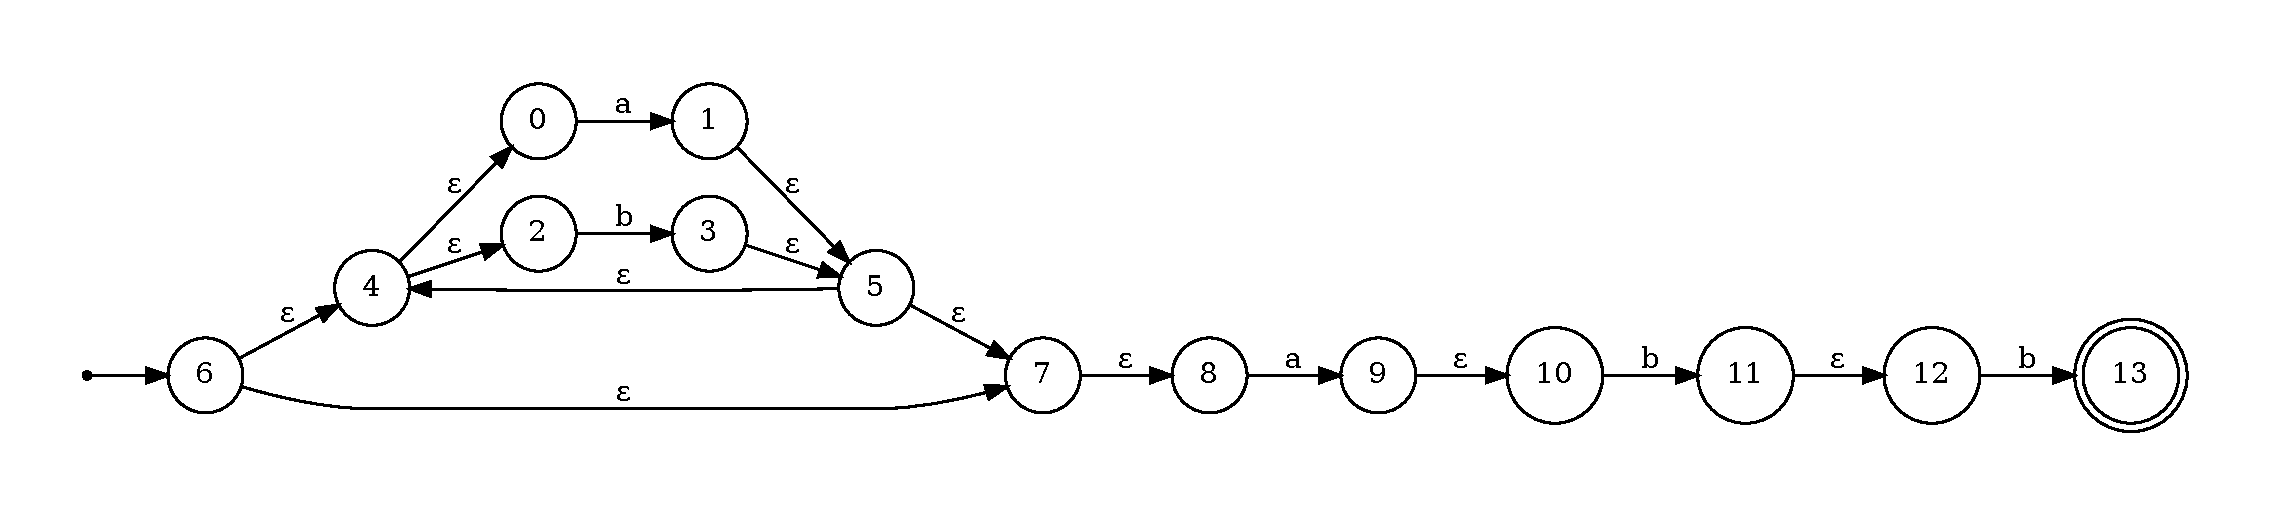
\includegraphics[width=0.9\linewidth]{figures/abb.pdf}
\caption{\code{(a|b)*abb} : 14 états $= 2n$ ($n = 7$).}
\end{figure}

\begin{figure}[H]
\centering
\begin{minipage}[b]{0.48\linewidth}\centering
  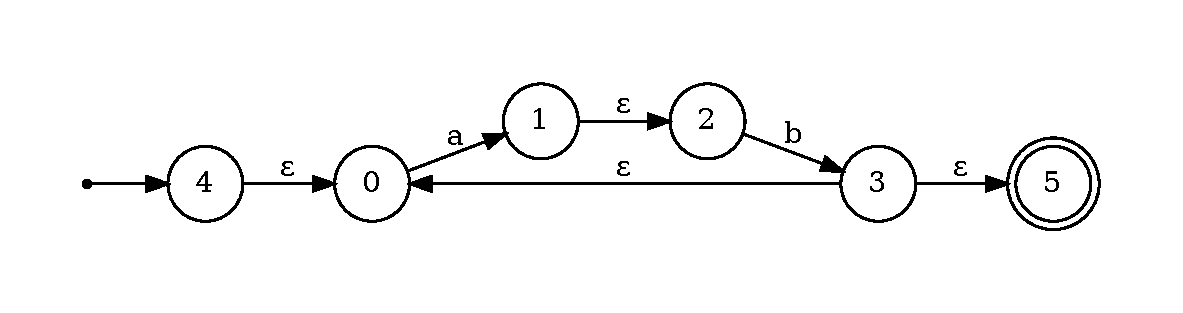
\includegraphics[width=\linewidth]{figures/ab_plus.pdf}
  \caption{\code{(ab)+} : 6 états.}
\end{minipage}\hfill
\begin{minipage}[b]{0.48\linewidth}\centering
  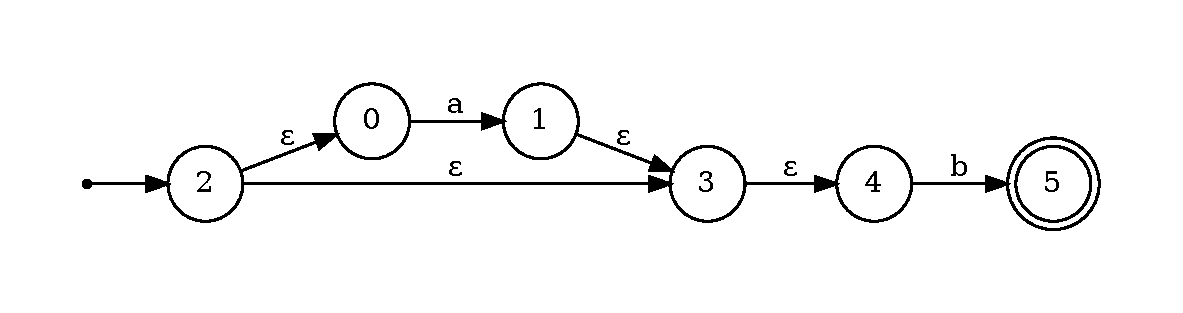
\includegraphics[width=\linewidth]{figures/a_opt_b.pdf}
  \caption{\code{a?b} : 6 états.}
\end{minipage}
\end{figure}

Dans \code{(a|b)*abb}, l'union \fr45 est construite en premier (ordre postfixe), puis l'étoile
\fr67 ($5 \to 4$ répète, $6 \to 7$ accepte zéro occurrence). Dans \code{(ab)+}, \code{ab} $= \fr03$ n'est pas recopié : la
boucle $3 \to 0$ répète et l'absence d'arête $4 \to 5$ exclut le mot vide. Dans \code{a?b},
l'arête $2 \to 3$ contourne \code{a} et l'absence de boucle exclut \code{aab}.

% ================================================================ TESTS
\section{Jeu de tests}\label{sec:tests}

\code{tests/tests.txt} suit le format \code{expression ; acceptés ; rejetés} (\tok{@} : mot vide) ;
un test d'erreur s'écrit \code{expression ; ERREUR ; position}. \code{python3 tests/run\_tests.py}
vérifie les mots, la borne $2n$, la numérotation $0..2n-1$ et l'invariant de Thompson. Le fichier
contient les 9 expressions imposées, nos 3 inventions, 6 cas complémentaires (priorités,
associativité, alphabet complet) et 10 tests d'erreur, dont les six de l'énoncé. Nos trois
expressions :
\begin{itemize}
\item \textbf{\texttt{(ab+)?}} : \tok{+} dans \tok{?} vérifie que chaque opérateur respecte
  l'invariant appliqué au résultat d'un autre ; c'est le cas qui a révélé le défaut
  (\code{b} accepté à tort).
\item \textbf{\texttt{a*+?}} : postfixés enchaînés, valides d'après l'énoncé ; teste la boucle
  $F' \to \texttt{*}F' \mid \texttt{+}F' \mid \texttt{?}F'$ et l'attribut hérité de $F'$
  (langage $a^*$, 8 états).
\item \textbf{\texttt{((a*)*)*}} : cycles d'\eps{} emboîtés ; une \eps-fermeture sans
  mémorisation des états visités bouclerait.
\end{itemize}
Le script contrôle aussi 500 expressions aléatoires (graine 2026) et 6 cas extrêmes
(jusqu'à 40 étoiles imbriquées).
\textbf{Résultats : 28/28 tests et 506/506 expressions conformes.} Sur la première version de
\tok{+} et \tok{?}, le même script donne 23/28 et 428/506 : la borne $2n$ était respectée, c'est le
contrôle de l'invariant qui révèle le défaut.

% ================================================================ DIFFICULTÉS
\section{Difficultés rencontrées et choix de conception}\label{sec:difficultes}

\begin{itemize}
\item \textbf{\texttt{+} et \texttt{?} sans nouveaux états.} La première version ajoutait
  seulement $\mathrm{fin}(r) \to \mathrm{init}(r)$ pour \tok{+} et
  $\mathrm{init}(r) \to \mathrm{fin}(r)$ pour \tok{?}. Après \code{b+}, l'état final de \code{b} a
  alors une transition sortante ; dans \code{(ab+)?}, l'arête $0 \to 3$ de \tok{?} entre dans la
  boucle de \code{b+} et le chemin
  $0 \xrightarrow{\varepsilon} 3 \xrightarrow{\varepsilon} 2 \xrightarrow{b} 3$ accepte
  \code{b}. Détecté en comparant les automates au langage attendu sur les mots de longueur
  $\le 4$ ; correction en section~\ref{sec:constructeurs}.
\item \textbf{Messages d'erreur.} Chaque test de jeton alimente l'ensemble \code{expected}, remis à
  zéro à chaque consommation : en cas d'échec, il donne exactement les jetons attendus.
\end{itemize}

% ================================================================ RESSOURCES
\section{Ressources externes}

\begin{itemize}
\item Support du cours ; Aho, Lam, Sethi, Ullman, \emph{Compilers: Principles, Techniques, and
  Tools}, 2006 (§3.7.4, §4.4, §5.5) ; documentation Graphviz.
\item \textbf{ChatGPT (OpenAI)}, consulté par Yahia Jaziri (Étudiant 3) pour clarifier la méthode
  de simulation, organiser la partie 5 et préparer des cas de test ; le code a été
  vérifié avec le jeu de tests.
\item \textbf{Claude (Anthropic)}, utilisé par Bara Mtawa (Étudiant 4) pour rédiger et mettre en
  forme ce rapport, redessiner la figure~\ref{fig:dep}, écrire le jeu de tests, \code{README.txt}
  et \code{EQUIPE.txt}, et vérifier les automates avec un script jetable (non rendu, module
  \code{re} comme oracle) qui a révélé le défaut de \tok{+} et \tok{?}, dont il a proposé le
  correctif. Une de ses erreurs dans les tests de \code{(a+b)?} a été repérée et corrigée.
\end{itemize}

\end{document}
